	%-----------------------------------------------------------------------------
%
%               Template for sigplanconf LaTeX Class
%
% Name:         sigplanconf-template.tex
%
% Purpose:      A template for sigplanconf.cls, which is a LaTeX 2e class
%               file for SIGPLAN conference proceedings.
%
% Guide:        Refer to "Author's Guide to the ACM SIGPLAN Class,"
%               sigplanconf-guide.pdf
%
% Author:       Paul C. Anagnostopoulos
%               Windfall Software
%               978 371-2316
%               paul@windfall.com
%
% Created:      15 February 2005
%
%-----------------------------------------------------------------------------


\documentclass[preprint,10pt,numbers]{sigplanconf}

% The following \documentclass options may be useful:

% preprint      Remove this option only once the paper is in final form.
% 10pt          To set in 10-point type instead of 9-point.
% 11pt          To set in 11-point type instead of 9-point.
% numbers       To obtain numeric citation style instead of author/year.

\usepackage{amsmath}

% non-template packages
\usepackage[bookmarks=true,pagebackref=false,pdftex]{hyperref}
\usepackage{epsfig} % eps figures
\usepackage{graphicx}
\usepackage[outdir=./]{epstopdf}
\usepackage{verbatim}
\usepackage{listings}
\usepackage{xcolor}

% Packages required for the tables
\usepackage{csvsimple}
\usepackage{booktabs}
\usepackage{multirow}
\usepackage{hhline}

\newcommand{\cL}{{\cal L}}


\begin{document}

\special{papersize=8.5in,11in}
\setlength{\pdfpageheight}{\paperheight}
\setlength{\pdfpagewidth}{\paperwidth}

\conferenceinfo{CONF 'yy}{Month d--d, 20yy, City, ST, Country}
\copyrightyear{20yy}
\copyrightdata{978-1-nnnn-nnnn-n/yy/mm}
\copyrightdoi{nnnnnnn.nnnnnnn}

\newcommand{\projectname}[0]{DangSan}
\newcommand{\freesentry}[0]{FreeSentry}
\newcommand{\dangnull}[0]{DangNull}
\newcommand{\metalloc}[0]{METAlloc} % Used this name from the published paper.

% Command to insert new line for table header
\newcommand{\tablecell}[1]{\bfseries \begin{tabular}{@{}l@{}} #1 \end{tabular}}

\lstset
{ %Formatting for code in appendix
    language=C,
    basicstyle=\footnotesize,
    numbers=left,
    stepnumber=1,
    showstringspaces=false,
    tabsize=2,
    breaklines=true,
    breakatwhitespace=false,
    %xleftmargin=.1\textwidth, 
    xrightmargin=.1\textwidth
}

% Uncomment the publication rights you want to use.
%\publicationrights{transferred}
%\publicationrights{licensed}     % this is the default
%\publicationrights{author-pays}

%\titlebanner{banner above paper title}        % These are ignored unless
\preprintfooter{Master Thesis Report}   % 'preprint' option specified.

%\title{DangSan: A mitigation technique to prevent dangling pointers exploit}
%\subtitle{Subtitle Text, if any}
%\title{DangSan: Practical Use-After-Free Detection}
\title{Efficiently Detecting Use-after-Free Exploits in Multi-Threaded Applications}
\authorinfo{Vinod Vijay Nigade}
           {Vrije Universiteit Amsterdam}
           {vinod.nigade@gmail.com}
%\authorinfo{Author 1}
%			{University}
%			{author@email.com}	
%\authorinfo{}
%           {}
%           {}

\maketitle


%\category{CR-number}{subcategory}{third-level}
% general terms are not compulsory anymore,
% you may leave them out
%\terms
%term1, term2
%\keywords
%use-after-free, SPEC2006
\begin{abstract}

Many systems software security hardening solutions rely on the ability to look up
metadata for individual memory objects during the execution,
but state-of-the-art metadata management schemes incur significant lookup-time or allocation-time overheads and are unable to handle different memory objects (i.e., stack, heap, and global)
in a comprehensive and uniform manner.

We present \projectname{}, a new memory metadata management scheme which
addresses all the key limitations of existing solutions. Our design relies
on a compact memory shadowing scheme empowered by an alignment-based object allocation strategy. \projectname{}'s allocation strategy ensures that all the memory objects within a page share the same alignment class and each object is always allocated to use the largest alignment class possible. This strategy provides a fast alignment-based memory-to-metadata mapping, while minimizing metadata size and reducing memory fragmentation. We implemented and evaluated \projectname{} on Linux
and show that \projectname{} incurs just 1.2\% run-time performance overhead, paving the way for practical software security hardening in real-world deployment scenarios.
\looseness=-1
\end{abstract}

\section{Introduction}
%1) Problem, vulnerabilities and impact, 
Many system applications are written in unsafe languages like C/C++. These languages are mostly used to have explicit control over hardware interfaces for optimal performance. For example, pointers are used to have explicit control on memory management. However, incorrect use of explicit control can lead to security vulnerabilities. Pointers incorrect use may lead to memory corruption. Use of dangling pointer is one instance of incorrect behaviour. \\

%2)Use-After-Free vulnerability
% \textbf{Mention stats and impact of recently.}\\
Dangling pointer is a pointer that points to the freed object. Use of dangling pointers i.e. Use-after-Free or Double-Free affects application integrity, availability and confidentiality~\cite{CVEMitre}. Dangling pointer may write invalid data into newly allocated memory resulting into data corruption, thereby affecting integrity. Memory allocators consolidate two adjacent freed chunks into single big chunk. When Use-after-Free occurs after chunk consolidation, invalid data can be used as chunk information. This state results into free-list corruption that can lead to application crash, thereby affecting availability. Moreover, Use-after-Free before chunk consolidation is prone to arbitrary code execution, thereby affecting confidentiality. Segmentation fault due to Use-after-Free can leak memory addresses, thereby making Address Space Randomization (ASLR) protection weak ~\cite{serna2012info}. Also, Use-after-Free vulnerabilities are reported and exploited in widely used browsers~\cite{tutorial2010internet, IRCVE}. Most of the highly critical vulnerabilities can be exploited with low complexity. The impact includes unauthorized information disclosure/~modification or service disruption ~\cite{NVDNist}. \\

%3) mitigation techniques
%\textbf{Undangle, Cling and other.Add techquines that are used in the past to mitigate dangling pointers exploit.}
% WE should mention what is pointer-object relationship briefy. with common development practice is to set NULL.s 
Common defensive coding practice is to set dangling pointer to benign value \texttt{NULL}. Manually, this practice is not scalable in large code base when multiple pointer copies are present. Same technique can be used dynamically to track all pointers to the object and set pointer value to \texttt{NULL} when object is freed. State-of-the-art mitigation techniques like \dangnull{} ~\cite{lee2015dangnull}, \freesentry{}~\cite{younan2015freesentry} tracks pointer-object relationship dynamically (during run-time). Compiler infrastructure like CIL ~\cite{necula2002cil}, LLVM~\cite{lattner2004llvm} is used to insert run-time pointer tracking functions. \dangnull{} uses red-black tree data structure to store and retrieve metadata (i.e. pointer-object relationship). It provides thread-safety for data structure operations using mutexes. However, \dangnull{} incurs high average performance overhead of $80\%$. Also, it does not track stack and global pointers. \freesentry{} has an average performance overhead of $25\%$. This performance is reported using CIL for static instrumentation. Performance numbers with LLVM are higher than CIL~\cite{freesentrypppt}. \freesentry{} uses hash-table to store and retrieve metadata. However, thread-safety for data structure protection is missing in \freesentry{}. Thus, it can break multi-threaded (production) applications. Also, \freesentry{} has not evaluated throughput degradation of web-servers. Therefore, state-of-the-art mitigation techniques either incur high performance overhead or have limited applicability. \\% Should we write missing throughput numbers for webservers

%4) Brief about first design 
In dynamic analysis, pointer-object relationship is tracked. To store and retrieve relationship information, we need highly efficient and complete shadow memory management framework. It should have low lookup and memory overhead. \metalloc{} ~\cite{istvan2016metalloc} is an efficient metadata management scheme. We first evaluated effectiveness of metadata management framework, \metalloc{}. We implemented \freesentry{} scheme using \metalloc{}. We found that thread-safety (i.e. data structure protection) introduces huge performance overhead of $70\%$. Applications in production environment are highly multi-threaded. We have proposed simple and fast lock-less Use-after-Free detection scheme, called as \projectname{} to protect multi-threaded applications efficiently. \projectname{} maintains per-Thread and per-Object metadata, thereby it reduces thread synchronization. We implemented \projectname{} using \metalloc{}. \projectname{} has moderate run-time overhead of $43.9\%$ when only heap pointers are tracked. Moreover, it introduces only $4\%$ more overhead when all pointers are tracked (Stack, Heap and Global).

\section{Background}
%TODO add some diagrams to explain more on this
%TODO every paragraph should have heading like DangNull.

% Dangling pointer information.
Dangling pointer is created when the memory object is freed. Dangling pointer is exploitable only when it is accessed. Moreover, attacker needs control over the freed memory where dangling pointer points. Attacker can place desired data in the controlled freed memory. Based on the context in which dangling pointer is used, a particular exploit can be triggered~\cite{CVEMitre, NVDNist}. The time between dangling pointer creation and use is highly important for the exploit. Longer the time period, more the chances to exploit~\cite{danglingptrfun, caballero2012undangle}.  Double free is a variation of use-after-free. Double free may corrupt memory allocator chunk information making system vulnerable. Dangling pointers are highly severe than spatial memory errors like, buffer overflow. Much of the research has happened to develop sophisticated buffer overflow mitigation techniques. Thus, spatial memory error vulnerabilities are hard to exploit. Due to this, dangling pointer vulnerabilities have gained popularity among attackers. However, mitigation techniques for dangling pointers are incomplete or incur high performance overhead. \\

% Mitigation technique : Static and dynamic analysis and its drawback.
Mitigation techniques include static analysis or run-time analysis. Static analysis   on the source code or binary is hard~\cite{feist2014statically}. It needs precise points-to analysis, type information, inter-procedural analysis. Moreover, object allocation, pointer propagation and object deallocation can occur at different places (functions, modules, threads) in the code. This further adds complexity to find accurate dangling pointers. On the other hand, dynamic analysis build pointer-object relationship during run-time. Pointer-object relationship is stored in object metadata (shadow object). Although, dynamic analysis is more accurate (low false positive and false negative rate) than static analysis, it incurs high performance overhead. Mostly, metadata lookups (i.e. finding metadata given an object or a pointer) are costly. \\

% Dynamic analysis: Why metadata management is required.
Dynamic analysis technique requires extra memory. This memory stores metadata associated with objects. Most of the schemes require object or pointer to metadata lookup. Metadata lookup should efficiently support object range lookups (i.e. finding metadata given any inbound object address). \dangnull{} uses variant of red-black tree to store metadata. Tree node is a shadow object associated with an object. Every node stores root address and size information. This bound information is needed for fast range lookups. However, metadata lookup time is highly variable. That is, it depends on the height of the shadow tree. On the other hand, \freesentry{} uses label based system~\cite{younan2010paricheck}. Label based system store unique labels in the shadow memory for each fixed size object field. Object may have multiple fixed size entries in the label table. Each entry will have same label. During metadata lookup, unique label is searched in the label table. This unique label is used as index in the object lookup hash table. However, \freesentry{} need to store more than one objects per entry in the object lookup table. Therefore, it may also have variable lookup time for the object metadata. \\

% Second data structure explanation.
Furthermore, pointer to object metadata lookup is required during pointer propagation (i.e. tracking pointer information in object metadata). \dangnull{} stores incoming and outgoing links in the shadow node along with bound information. Incoming link denotes that the object is pointed by other object and outgoing link denotes that the object is pointing to other object. \dangnull{} retrieves shadow object representing pointer address. It checks and modifies outgoing link of this object to point to other shadow object (i.e. to the object pointed by the pointer). Similarly, it modifies incoming link of the other shadow object. It has variable metadata retrieval time. \freesentry{} uses pointer lookup hash table to retrieve pointer information. Pointer lookup table does not require range lookups. Thus, hashtable is a valid choice. \freesentry{} requires huge memory for label table (almost equal to process memory), object and pointer lookup tables. Moreover, shadow memory data structure has to be thread-safe. Large number of pointer propagations, object allocations and deallocations in multi-threaded application will drastically slow down application performance. Thus, synchronizing operations on data structures increase performance overhead. \dangnull{} protects data structure using mutexes. However, \freesentry{} has not focussed on thread-safety. In \freesentry{}, object and pointer lookup hash tables need to be protected. This can be achieved having a coarse-grain or a fine-grain per-hash table entry lock.  \\

% 1) Explain metalloc. How it is suitable?. 
Any dangling pointer detection scheme (dynamic analysis) requires efficient metadata management (i.e. fast metadata allocation and retrieval strategy), thread-safety and low memory overhead. \metalloc{}~\cite{istvan2016metalloc} is an efficient and practical memory shadowing framework. It is based on the strategy that every object in the same memory page has same alignment. Thus, it maintains metadata information per page instead of per memory object. Given a pointer, it first finds corresponding page information i.e. metadata base address and alignment information. Next, it  calculates pointer offset within the page. The offset and alignment information is used to find corresponding entry in the metadata area. Therefore, it has fixed metadata lookup time for any object address range. Moreover, it provides uniform metadata tracking for all the objects (Heap, Stack and Global). Most importantly, it incurs only $1.2\%$ average run-time performance overhead for SPEC2006 benchmarks. Low performance overhead and memory optimized design along with easy to use framework makes \metalloc{} an ideal choice for implementing dangling pointer prevention scheme. \\

% 2) How freesentry desing can be achieved.
We implemented \freesentry{} scheme using \metalloc{}. \metalloc{} provides efficient object-to-metadata mapping. Therefore, we do not need Label table to fetch metadata associated with the objects. Object metadata stores a pointer to the pointer list (i.e. list of pointers information that are pointing to the object). Thus, we do not need object lookup table. Fetching a pointer information corresponding to an object requires fixed retrieval time. Next, we use pointer lookup hash table similar to \freesentry{}. Pointer-to-object metadata is retrieved using pointer lookup table. Each entry in the pointer lookup table is a doubly list of pointer information. This pointer information is also a node in the object metadata list. Thus, given a pointer, fetching an object pointer list is just finding the correct pointer information in the pointer lookup table. We evaluated this design for SPEC2006 benchmarks. We performed experiments on $64$-bit CentOS Linux with Intel Xeon CPU E5-$2640$ v$3$. We implemented LLVM compiler pass to insert run-time pointer tracking function. \\ 

\begin{figure}[t]
\center
  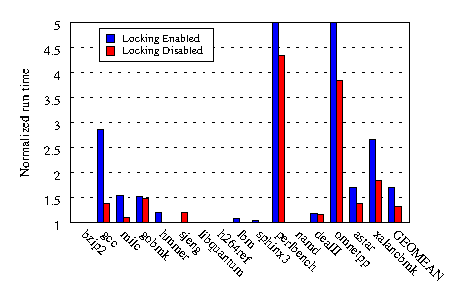
\includegraphics[width=3in]{plots/metalloc_freesentry.eps}
  \caption{SPEC2006 performance overhead for \freesentry{} scheme using \metalloc{}. Locking enabled and disabled represents normalized numbers with and without thread-safety, respectively.}
  \label{fig:metalloc-freesentry-graph}
  \vspace{-1em}
\end{figure} 

Figure~\ref{fig:metalloc-freesentry-graph}\ shows SPEC2006 run-time overhead for \freesentry{} design using \metalloc{}. It depicts normalized (with baseline) numbers with and without thread-safety. With thread-safety, run-time overhead on an average (geometric mean) is $69.6\%$. We used pthread mutexes to protect object pointer list and pointer lookup table. Without thread-safety, run-time overhead is just $33.2\%$. This number matches with the average \freesentry{} performance overhead when implemented on LLVM~\cite{freesentrypppt}. However, all our bechmarks are SPEC2006 whereas \freesentry{} has mix of SPEC2000 and SPEC2006. Moreover, our average number includes \texttt{omnetpp} run-time which has huge overhead. That is, \texttt{omnetpp} number further increases average value compared to \freesentry{}. In conclusion, \metalloc{} seem to perform better than Label based system used in \freesentry{}. Also, it has low memory overhead. However, introducing thread-safety dramatically increases performance overhead, making it impractical in production environment.
% 3) Explain graph.
% 4) Explain need for other design. 



\section{Overview} \label{Overview}

Large number of object allocations, deallocations and pointer propagations pose challenges in developing fast Use-after-Free detection system. Large scale applications like Web-Servers, Browsers are multi-threaded applications. Using dynamic analysis efficiently in multi-threaded application requires less thread synchronization. Recently proposed Use-after-Free detection systems introduce huge performance overhead or they have ignored thread-safety completely. \\

In this paper, we present and evaluate \projectname{}, a simple and efficient system to prevent Use-after-Free exploits during run-time. LLVM compiler instrumentation pass is used to insert run-time tracking function calls. We present optimal run-time data structure design for multi-threaded application. It removes a need for thread synchronization. We show that this lock-less design can be used practically in production servers that needs low overhead. \\
 
This paper has following contribution,
\begin{itemize}
\item We show that thread-safe Use-after-Free schemes in multi-threaded application can lead to huge run-time overhead. We implemented \freesentry{} scheme using \metalloc{}. We evaluated this design with and with-out thread-safety.
\item We propose \projectname{}, a novel, simple and efficient lock-less system to efficiently store and retrieve pointer-object relationship in Multi-threaded applications.
\item We implemented and evaluated \projectname{} for SPEC2006 CPU benchmarks and widely used Web Servers (\texttt{httpd}, \texttt{nginx} and, \texttt{lighttpd}).
\item We verified \projectname{} correctness on recently discovered Use-after-Free (and Double-Free) vulnerabilities.
\end{itemize}

Section~\ref{\projectname{}}\ discusses \projectname{} design. It discusses design assumptions, criteria and parameters. Performance and correctness evaluation is presented in Section ~\ref{evaluation}. Related work is discussed in Section ~\ref{relatedwork}. Finally, Section ~\ref{conclusion} concludes our contribution. 


%\section{Motivation}
%5) Our Approach: Briefly
In this paper, we present and evaluate \projectname{}, a system to prevent dangling pointers during run-time. \projectname{} uses metadata management framework to track metadata associated with memory objects. We use LLVM static transformation pass to insert run-time function calls. Our design is based on per-Thread per-Object data structure. Thereby, it removes need for thread synchronization. This lock-less design is highly efficient in heavily multi-threaded applications like, Web Servers. \\
 
This paper has following contribution,
\begin{itemize}
\item We evaluated effectiveness of \metalloc{} framework by implementing dangling pointer prevention. Design is similar to \cite{FreeSentry}. We show that thread synchronization may lead to huge degradation.
\item We propose \projectname{}, a unique lock-less system design to invalidate dangling pointers during run-time.
\item We implemented and evaluated \projectname{} on SPECint2006 CPU benchmarks and, widely used Web Servers (i.e. httpd, nginx and, lighttpd).
\item We evaluated \projectname{} for correctness on recently discovered use-after-free(and double-free) vulnerabilities.
\end{itemize}

This paper is organized as follows. Section II shows the effectiveness of \metalloc{} framework for preventing dangling pointers. Section III discusses our novel lock-less \projectname{} design. Also, it discusses design decision criteria and parameters. Section IV presents \projectname{} implementation and issues faced. Next, Section V evaluates \projectname{} in terms of performance and correctness. Related work is discussed in Section VI. Finally, Section VII concludes our contribution.

%1) Instrumentation phase
%2) Implementation of run-time using FreeSentry approach
%3) Comparison of with lock and without lock
%4) Need to go for other approaches

%1) Talk about dangling pointer creation.
Dangling pointer is created when the object is freed and pointer still has reference to it. Use of dangling pointer leads to undefined behaviour, mostly segmentation fault. Normally, developers set pointers value to NULL after object free. Applications have NULL check which prevents invalid dereferencing of dangling pointers. However, manually this technique is not scalable (feasible) when multiple pointer copies are present. Thus, We need metadata to keep track of almost all pointers pointing to the object during run-time. \metalloc{} is an efficient metadata management framework implemented on top of custom allocator, \texttt{tcmalloc}. We first implemented a pointer tracking scheme similar to \freesentry{} using \metalloc{}. To maintain object-to-metadata mappings, \freesentry{} uses label based system whereas \metalloc{} uses \textit{metapage table} (a hash table). This data structure should efficiently retrieve metadata given any inbound address to the object. To retrieve pointer-to-object metadata, we use a hash-table called as pointer lookup table. Figure~\ref{fig:metalloc-freesentry} shows new pointer tracking scheme based on \metalloc{}.\\

%\begin{figure}[t]
%\center
%  \includegraphics[width=2.8in,height=2.4in,keepaspectratio]{figures/metalloc-%freesentry.eps}
  %\caption{ Dangling pointer detection scheme based on \freesentry{} using %\metalloc{}.}
 % \label{fig:metalloc-freesentry}
 % \vspace{-1em}
%\end{figure}

\textbf{Implementation.} We maintain per object a structure called as headnode. It contains a unique identifier (ID) that determines the liveness of the object, a lock to protect pointer list, a pointer to the doubly pointer list and a MAGIC field. MAGIC field is a XOR result of ID and a Constant. \metalloc{} allocates headnode for every possible object (Global, Stack and Heap). It initializes headnode with zero. \metalloc{} metadata retrieval function returns pointer to the headnode. This return value can be NULL, garbage or a valid headnode. Thus, validity of the object is confirmed using MAGIC field. Moreover, tracking for stack objects and pointers can be skipped during run-time using MAGIC field. Also, tracking of global objects (not pointers) are skipped  by reserving lower 16 bits of identifier only for the global objects. It is assumed that total number of global objects during a run remains constant and less than $2^{16}$.  \\

Pointer information is tracked in a structure called as ptrnode. Each ptrnode contains, pointer address to invalidate, pointer value to check if pointer still points to the object, object ID in which pointer resides to check the validity of the pointer object, backward and forward pointers to iterate through doubly list.
Pointer lookup table gives mapping from pointer address to the pointer information. Each $8$ byte pointer contains a slot in the pointer lookup table. As size of pointer lookup table is limited, collision is handled through chained doubly linked list. When number of pointer traces increases, length of doubly linked list increases. Application runtime overhead increases dramatically when linked list traversal increases. Thus, pointer lookup table size should be selected wisely. \\

%2) Static instrumentation
\textbf{Static Instrumentation.} We use LLVM-based static instrumentation to insert run-time tracking functions. We have not instrumented any allocation (malloc, calloc, realloc, new) and deallocation (free, delete) calls. \metalloc{} provides a way to insert hook before or after allocation(deallocation routine). We have enabled hook after allocation routine and before free routine. These hooks initialize metadata and invalidate pointers from pointer list, respectively. We are only interested in pointer assignments. 
$$ store\ rhs,\ lhs $$
We wrote a function pass to track interested store LLVM IR instructions. We track only those store instructions where \textit{rhs} is a pointer type. Stack pointers are live only for the function scope. Also, we are not tracking stack objects. We conservatively filter out stores when \textit{lhs} or \textit{rhs} is a stack object. Moreover, incorrectly instrumented stack objects and address are skipped during run-time. We also skip stores when \textit{rhs} is a global object, a function pointer or a constant null pointer. We insert run-time tracking routine after store instruction in this design. However, in \projectname{} we insert it before store instruction. This is to check the old value of the pointer. \\

\textbf{Backward Compatibility.} Pointer invalidation by value NULL can break application backward compatibility. Many applications use freed object address as a numerical value to calculate relative offset or number of unit size elements. Setting pointer value to NULL will result into incorrect and undefined behaviour. To solve this problem, we invalidate pointer value by setting the most significant bit to $1$. On Linux $64$-bit this invalid address results into kernel address space. Next, some pointers can point out-of-bound. STL vector in C++ stores three fields, $1)$ Start of array $2)$ Next empty location in the array $3)$ End of array. Here, End of array points to one byte off the object bound. We register pointer by using pointer value to find the metadata. Thus, off-by-one object address will end up registering pointer into wrong object's metadata. To solve this problem, we increase the size of the requested memory during allocation by $1$. Also, we found a weird pointer usage in $gcc$. SPECint2006 $gcc$ allocates a memory and stores allocated address minus some constant value into the pointer. Registration of this pointer ends up in wrong object's metatdata. We handled this as a special case during static instrumentation. We register object root pointer when \textit{rsh} is GEP LLVM instruction and GEP indices operand is negative or SUB LLVM instruction. \\

%\begin{figure}[t]
%\center
%  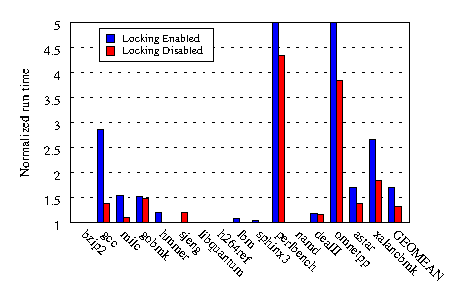
\includegraphics[width=3in]{plots/metalloc_freesentry.eps}
%  \caption{SPECint2006 performance overhead of dangling pointer prevention using %\metalloc{}. Locking enabled represents with thread synchronization and Locking %disabled represents without thread synchronization.}
%  \label{fig:metalloc-freesentry-graph}
%  \vspace{-1em}
%\end{figure} 

\textbf{Evaluation.} We instrumented SPECint2006 benchmarks with above pointer detection scheme. Safestack option is enabled for baseline numbers. \metalloc{} is implemented with \texttt{tcmalloc} custom dynamic memory allocator. We performed experiments on 64-bits CentOS Linux with Intel Xeon CPU E5-2640 v3. Figure~\ref{fig:metalloc-freesentry-graph} shows SPECint2006 runtime overhead with and without thread synchronization. With locking enabled, \texttt{perlbench} and \texttt{omnetpp} has normalized runtime degradation of more than $5x$ ($12x$ and $7x$ respectively). With thread synchronization, runtime overhead compared to baseline-safestack is $69.6$\% and without thread synchronization is $33.2$\%. We have used pthread mutex per memory object and a global pthread read-write lock for pointer lookup table protection. Also, pthread spinlock is used for assigning object identifiers. Out of three locks, pointer lookup table is highly contented. So, locking contributes huge performance degradation. \freesentry{} experiments only with single threaded applications. It has used no locks. We cannot directly compare performance of our design with \freesentry{}. Because, number of instrumentation and implementation may differ in both design. Moreover, \dangnull{} which uses pthread mutexes to protect its internal data structure has on average runtime overhead of $80$\%. Locking overhead is one of the reason in \dangnull{}. This problem has motivated to go for \projectname{}, a novel lock-less system to prevent dangling pointers in multi-threaded application.


\section{\projectname{} Design} \label{\projectname{}}
Data structure thread-safety in multi-threaded application introduces huge overhead. Efficient design should reduce concurrent access to data structure. In a simple design, we just need a list of pointers to the object. When object is freed, pointers are read from the list and invalidated. This simple design has following issues in multi-threaded environment. $1)$ Multiple threads writing to the same object list need to synchronized (i.e. object to metadata lookup need to be synchronized). $2)$ When pointer is no longer pointing to the same 
object, it should be removed from the list. Pointer to object metadata lookup is used to remove pointer information from the object metadata. Therefore, pointer to object metadata lookup need to be synchronized. $3)$ Same pointer can be inserted multiple times in the object list. \dangnull{} and \freesentry{} maintains pointer-object relationship. Relationship information does not change when pointer keeps pointing to the same earlier object. When pointer points to a new object, old relationship is removed and new relationship is inserted. Therefore, we need thread synchronization for object to metadata and pointer to metadata access. \\% We need to protect concurrent access when objecct to data structure looku and pointer to object lookup. % We need  

Pointer remains in the old object list even after it no longer points to the object. This can lead to incorrect pointer invalidation when old object is freed. Pointer value can be checked to prevent incorrect pointer invalidation. Pointer is invalidated only when pointer points to any inbound object address. The same technique is needed when pointer is modified in non-instrumented code. We do not need pointer to object metadata. Also, removal of old pointer-object relationship adds extra performance overhead. Therefore, pointer to object lookup can be skipped, thereby removes need for a thread synchronization. Concurrent access to per object metadata (list) cannot be skipped. In a simple design, pointer list per object is required. Pointer list is equivalent to a log of pointers. Now, reducing concurrent access to pointer list per object boils down to a well-known problem of concurrent logs. Mostly, concurrent logging is on per-Thread basis. Concurrent logs are write efficient but with costly reads. \\

Normally, number of pointer propagations are higher than the number of object allocations and deallocations. Therefore, pointer propagation tracking should be efficient. One approach is to  skip pointer-to-object metadata lookup. That is no need to maintain old pointer-object relationship. This operation is equivalent to log-write. Motivated by the fact that log-write is efficient, we designed per-Thread per-object log data structure to track pointers pointing to the object in the log. Log read is required when object is freed. The design is similar to a log-structured file system \cite{rosenblum1991design} that maintains circular buffer to track I/Os. The design rationale behind \projectname{} is that the number of pointer registrations (write) are higher than the number of objects free (reads).

\begin{figure}[t]
\center
  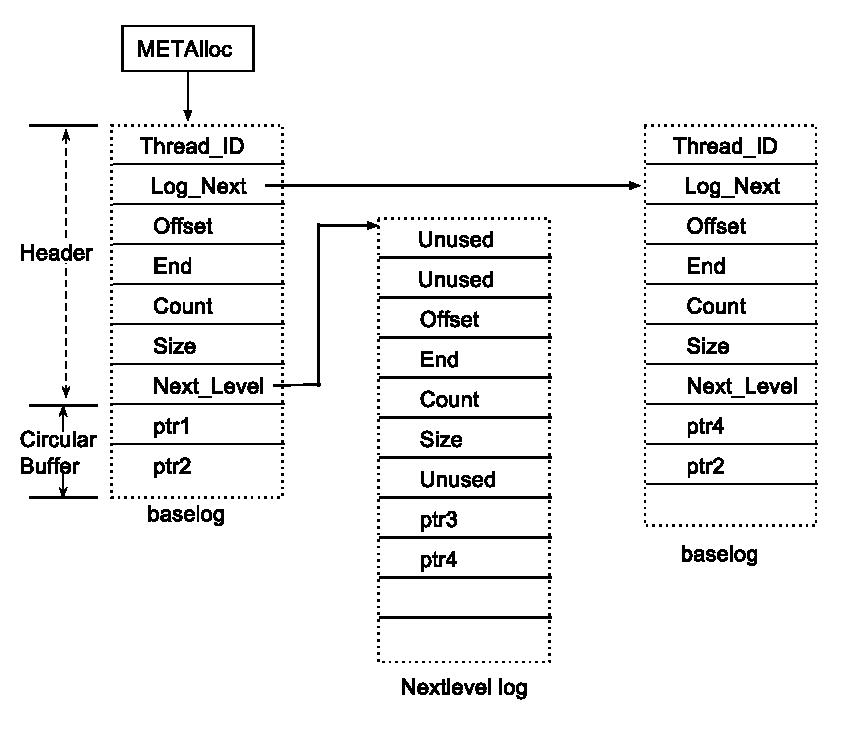
\includegraphics[width=2.8in,height=2.4in,keepaspectratio]{figures/dangsang_design.eps}
  \caption{DangSan data structures for two threaded application.}
  \label{fig:dangsang_design}
  %\vspace*{3in}
  \vspace{-1em}
\end{figure}

\subsection{System Overview}
Figure~\ref{fig:dangsang_design} shows \projectname{} design. Every object metadata has per-thread log. As we are not maintaining pointer-object relationship, only pointer address is needed and stored in the log. Object to metadata lookup retrieves corresponding log for a thread. Pointer tracking function retrieves corresponding log and writes pointer address into it. When object is freed, all per-Thread logs are retrieved. Pointer addresses are read from all the logs and invalidated. During invalidation, current value of pointer is read and checked to see whether it still points to the object. \\  

% Issues: Thread ID, per thread storage
\textbf{per-Thread Storage.} 
We need efficient retrieval of per-Thread log for a given object. One approach is to maintain object lookup table per-Thread. Similar to global shadow memory technique, it should also support range queries. Moreover, maintaining per-Thread object lookup table will incur huge memory overhead. Second approach is shown in Figure~\ref{fig:dangsang_design}, where per-Thread log is maintained in global object list. Maintaining global object list (dynamically) needs thread synchronisation. Another approach is to maintain a static array of log pointers per object. Thread specific \emph{ID} can be used as index into the static array to retrieve corresponding log. Though this approach uses fast array indexing, it has high memory requirements. Second approach is memory efficient but needs concurrent access support. Log removal from dynamic object list is needed only during object free and not during pointer propagation or object allocation. Therefore, only concurrent insertions and reads are needed during pointer propagation. Lock-free insertions and reads can be achieved through compare and swap (\emph{CAS}) atomic instruction~\cite{valois1995lock}. Unique thread IDs can be used to identify thread log. One can use thread IDs assigned by the run-time system or maintain own thread IDs. Maintaining own thread IDs can help in reusing IDs. Reusing thread ID helps in reusing thread log. Dynamic object list can grow large when application has too many short lived threads. Thus, reusing thread log is necessary to reduce list traversal. \\ % explain why only insertion is needed % Mention about per thread storage for each objects metadata. We will need then metadata tracking for perThread. It is not global, which will waste memory.


% Issues: Log Overflow
\textbf{Log Overflow.} 
 In \projectname{}, pointer-object relationship is not maintained. That is, pointer addresses are not removed from old object logs. Depending upon the number of pointers to the object per thread, log overflow has to be handled. One approach is to reallocate log with larger size. But, reallocated log address can be different than the old log address. We need deletion operation to modify dynamic list with this new log address. That is, \emph{CAS} atomic instruction for thread-safety can no longer be used easily. Second approach is to allocate new log for the thread and invalidate old log. Log invalidation is performed simply by setting thread ID maintained in the log to an invalid value. This way, thread can retrieve only a new log using thread ID. However, this approach increases length of dynamic list, thereby increases log retrieval time. Another approach is to introduce second level indirect log. Concurrent access is required for base level logs. Figure~\ref{fig:dangsang_design} shows Second level log. It is activated only when the base level log overflows. After base log overflows, each thread will find base log first and then second level log to store  pointer address. %TODO insted of store pointer address, use register pointer address.
Similar to base log, second level log can overflow. This can be handled easily by reallocating second level log with larger size. This operation does not require thread synchronization.  \\
% No information of pointer-object relationship. Increases pointers per logs. Duplicate pointers.
% Reallocating log is not possible because of deletion operation it involves.

We have introduced few terms in our context $1)$ \textit{Unique pointer:}  Pointer address is stored only once in the log (i.e. Pointer has only one entry in the log). $2)$ \textit{Duplicate pointer:} Pointer address is stored more than once in the log (i.e. Pointer has more than one entry in the log) $3)$ \textit{Stale pointer:} A stored pointer in the log that no longer points to the object. $4)$ \textit{Valid pointer:} A stored pointer in the log that points to the object. Choice of second level data structure also depends on the number of \textit{Unique pointers} and \textit{Duplicate pointers}. Hashtable can be used when \textit{Duplicate} pointers are higher than the \textit{Unique} pointers. But, HashTable introduces huge memory wastage.\\

%TODO use this statement in garbage collection.
%Moreover, Garbage collection of \textit{Stale pointers} is required when it dominates the log. It frees some space from the data structure. Intuitively, on a time scale, old pointers tend to have invalid values than the recent pointer. Hastable cannot track pointer registration history. Thus, Circular log seems the best choice for the stale pointers removal.\\

% N-Lookbehind
\textbf{N-Lookbehind.} 
% Why N-Lookbehind? Duplicates are removed. As we are not keeping pointer-object relationship, we need to removed duplicate pointers from the object log.
One of the reason for log overflow is large number of \textit{Duplicate} pointers. One approach to remove duplicate pointers is to look-behind in the log for a pointer i.e. check pointer address against all stored pointers. Checking entire log for \textit{Duplicate} pointers is a heavy operation. However, we can lookbehind \emph{N} last offsets and skip pointer registration when pointer is within N-Lookbehind offset in the log. Normally, the same pointer is used to iterate over the object memory. This iteration occurs within a short period of time (e.g. in the loop). Depending on the value of $N$, we can eliminate large number of duplicate pointers. In normal scenario, \textit{Unique} pointers are less than or equal to object size. When log size grows larger than object size, \textit{Duplicate} and/or \textit{Stale} pointers are higher than \textit{Unique} pointers. Selection of \emph{N} value is critical in removing \emph{Duplicate} pointers but by considering performance overhead. \\

\begin{figure}[t]
\center
  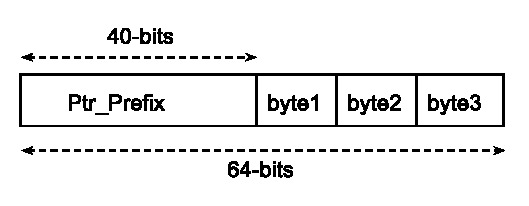
\includegraphics[width=2.8in,height=2.4in,keepaspectratio]{figures/pointer-entry.eps}
  \caption{Pointer entry in the log, where Ptr\_Prefix is a pointer value from 48-bits to 8-bits and byte is a lowermost byte of the pointer}
  \label{fig:pointer_entry}
  %\vspace*{3in}
  \vspace{-1em}
\end{figure}  

Moreover, \emph{N}-Lookbehind can be used to increase log size utilization. On $64$-bit architecture, only lower $48$-bits represent user space virtual memory address. That is, upper most $16$-bits are not used. These two bytes can be used to store two more pointers i.e. (three pointers per log slot). Figure~\ref{fig:pointer_entry} shows a technique to make use of two bytes. We store all three pointers when $40$-bit prefix of all pointers is same. In other word, pointers differing only in lowermost byte can be stored together in the same log slot. Store $40$-bit pointer prefix in the uppermost $40$-bit of the log slot. Next, three remaining lowermost bytes (\textit{byte1}, \textit{byte2}, \textit{byte3}) of the log slot are used to store lowermost byte of three pointers.
Therefore, pointers within $256$ bytes range occupy the same slot in log. Here, \emph{N}-Lookbehind is used to find a log slot where pointer prefix and a log slot prefix match. Following steps can be used to insert pointer into the log, $1)$ Find the empty slot by matching pointer prefix within \emph{N}-Lookbehind entries. Matched slot is empty only when \textit{byte2} or \textit{byte3} is zero ($0x00$). $2)$ When empty slot is found, insert lowermost pointer byte at empty byte location. When pointer lowermost byte is $0x00$, swap this value with $byte1$. That is, pointer byte $0x00$ will always be stored at $byte1$ location. This is because, $0x00$ value denotes empty byte location. $3)$ Skip the registration when \textit{Duplicate} pointer (i.e. both prefix and a byte matched) entry is found. $4)$ When no matching log slot is found, insert $48$ pointer bits into uppermost $48$-bit of new log slot. Thus, \emph{N}-Lookbehind strategy helps in comparing atmost $(N \times 3)$ pointers at the cost of \emph{N} sequential memory access. In best case, log utilization increases by the factor of $3$. \\

% Not sure if we can use this term.????
\textbf{Garbage Collection.} 
Another reason for log overflow is a large number of \textit{Stale} pointers. Normally, with the time, old stored pointers tend to become \textit{Stale}. One approach to remove \textit{Stale} pointers is to treat log as a circular buffer. When log is about to overflow, iterate from log end to \textit{Valid} pointer slot to find \textit{Stale} pointers. Modify log end value with new \textit{Valid} log slot. To determine pointer validity, read pointer value and check whether it still points to the object. For fast check, object bound information can be maintained in the object metadata. We need to grow the log when no \textit{Stale} pointer slot is garbage collected. Note, when we store three pointers per slot, log slot is stale only when all three pointers are stale. Due to garbage collection, amount of work is shifted from object free context to pointer registration context. Total work remains the same with and without garbage collection. Garbage collection avoids log overflow, thereby prevents log reallocation cost. \\

\textbf{Pointer Liveness.} 
\textit{Stale} pointers no longer point to the object. Object in which \textit{Stale} pointer resides may no longer be live (i.e. unmapped). Accessing non-live pointer results into segmentation fault. We access \textit{Stale} pointers in garbage collection and object free routines. To prevent invalid access to \textit{Stale} pointers, one approach is to introduce new action for \texttt{SIGSEGV} signal in garbage collection and object free routines. Ignore \texttt{SIGSEGV} when signal is generated in these routines. Restore old \texttt{SIGSEGV} signal action at the end of above mentioned routines. Another problem with \textit{Stale} pointers is that the pointer memory location might have been allocated to a new object. There exist a small window in object free routine between pointer value check and pointer invalidation operation. In this window, another application thread can write new value to the pointer which may get invalidated wrongly in object free routine. To avoid this problem, we use \emph{CAS} atomic instruction to perform pointer invalidation only when pointer value is old.

\subsection{Static Instrumentation}
Run-time tracking function is instrumented statically using LLVM. Only pointer propagations are tracked (i.e. run-time tracking function is inserted before or after pointer assignment instruction). Allocations (\texttt{malloc}, \texttt{realloc}, \texttt{calloc}, \texttt{new}) and deallocations (\texttt{delete}, \texttt{free}) instructions have to be intercepted if these routines cannot be hooked during run-time. Listing~\ref{lst:staticsrc}\ shows instrumented C code. Run-time tracking function \texttt{track\_ptr()} is inserted after object allocation and pointer propagation code statement (Line $6$ and $8$). \texttt{track\_ptr()} first retrieves metadata for an object and registers pointer address in the metadata. Similarly, \texttt{nullify\_ptr()} is inserted after object deallocation code statement (Line $10$). It retrieves object metadata and invalidates all stored pointer by setting pointer to benign value NULL.    

\lstinputlisting[float, caption=Static Instrumentation, numbers=right, language=C, label={lst:staticsrc}]{Source/static_reg.c} 

We are only interested in pointer assignments.
$$ store\ rhs,\ lhs $$
We track only those store instructions where \textit{rhs} is of pointer type. We pass both \textit{rhs} and \textit{lhs} as arguments to the run-time function. Stack objects are frequently created and destroyed. Benefit of tracking stack object compared to its performance overhead is very low. Similarly, global objects are destroyed (freed) only when application exit. Therefore, we conservatively filter out stores when \textit{rhs} is a stack or global object. Moreover, incorrectly instrumented stack or global objects are skipped during run-time. Also, We skip store instrumentation when $rhs$ is a function pointer or a constant null pointer. When old pointer value is needed in tracking function, insert run-time tracking function before store instruction.  \\

\subsection{Parameters Selection} 
% First discuss what parameters, how it affects performance, solution.
% In the last discuss, emprical results.
Performance of \projectname{} depends on the following three parameters. $1)$ \textbf{N-Lookbehind}: Increasing the value of \emph{N} decreases the number of \textit{Duplicate} pointers. It increases the chance of placing a pointer at already filled log slot. That is, it increases memory utilization of the log. However, increasing the value of \emph{N} introduces cost of reading sequential memory. Distribution of pointer patterns in the log is application specific. Thus, choice of selecting value $N$ depends on the application. $2)$ \textbf{Log Size}: Increasing the log size decreases the number of log reallocations. However, it increases memory wastage. Selection of baselog size (default log size for each thread) and reallocation strategy is critical in maintaining balance between performance overhead and memory wastage. One reallocation strategy is to increase log size additively. This will reduce memory wastage but may need large number of reallocations. Another approach is to increase log size exponentially. This require logarithmic steps to reach maximum needed memory for an object. We perform log resize operation only on the second level log. $3)$ \textbf{Thread-Specific operations}: Thread ID is maintained in thread-specific storage. Also, every log stores thread ID to identify thread-specific log. Maintaining and using thread-specific storage introduces extra memory access and computational checks. These extra performance overhead can be avoided for single threaded applications. One approach is to give compile time option to select the required variant (i.e. single threaded or multi-threaded). Another approach is to maintain thread ID in a register instead of thread-specific storage. Empirically for SPEC2006 benchmarks, $N = 3$ and baselog size $=\ 8$ (number of pointers) with exponential log resize gives better performance.
%TODO Hashtabel approach


%%%% Log size selection

%%%% Talk about the memory that we get for the \projectname{}
%%%% Single-Threaded v/s Multi-Threaded options. Selection of GS/FS register





\section{Implementation}
We implemented \projectname{} on linux with \metalloc{} (metadata management) and \texttt{tcmalloc} ~\cite{ghemawat2009tcmalloc} (custom memory allocator). Static instrumentation is built using LLVM $3.8$. We do not instrument (malloc, calloc, realloc, new) and deallocation (free, delete) function calls. \metalloc{} provides a way to insert custom hook before and/or after allocation (deallocation) functions. We instrument only pointer store instruction. Run-time tracking functionality is provided in a static library. \\

\textbf{Application Compatibility.}
We found that following cases can break application compatibility. $1)$ \textbf{Pointer subtraction}: Subtracting two dangling pointers pointing to the same object is a valid code statement. It can break due to \projectname{}. Our system sets pointer value to \texttt{NULL} when object is freed. Therefore, subtracting two dangling pointers result into $0$ (i.e. incorrect value). To solve this problem, we invalidate pointer by setting the most significant bit of pointer value to $1$. On Linux $64$-bit, this invalid pointer value points into kernel address space. $2)$ \textbf{Off-by-One byte}: Some valid pointers can point out-of-bound by one byte. For example, STL vector has three fields, \texttt{start}, \texttt{next} and \texttt{end}. \texttt{start} points to start of the array memory. \texttt{next} points to next empty array location. \texttt{end} points to end of the array memory. \texttt{next} and \texttt{end} can point out-of-bound by one byte. Therefore, these pointers will get registered for wrong object. When wrong object is freed, \texttt{next} and \texttt{end} pointers will get invalidated. To solve this problem, we increase object allocation size by one. $3)$ \textbf{GCC issue}: We found one weird pointer usage in SPEC2006 \texttt{gcc}. \texttt{gcc} allocates a memory and stores allocated address minus some constant value into the pointer (i.e. no root address is stored). Registration of this pointer happens for wrong object. This pointer usage is wrong. Thus, we handled this issue as a special case during static instrumentation. For \texttt{GEP} LLVM instruction, when indices operand is negative constant or \texttt{SUB} LLVM instruction, we take root address of the object.


\section{Evaluation} \label{evaluation}
\begin{table}[t]
	\begin{tabular}{l*{4}{c}}
		\toprule
		\multirow{2}{*}{\bfseries Benchmarks} & \multicolumn{2}{c}{\bfseries \begin{tabular}{@{}l@{}} Normalized \\ with Baseline \end{tabular}} & \multicolumn{2}{c}{\bfseries \begin{tabular}{@{}l@{}} Normalized \\ with SafeStack \end{tabular}} \\%& \multirow{2}{*}{\bfseries \begin{tabular}{@{}l@{}} Number of tracking \\ functions inserted \end{tabular}} \\ % Great ;) hack to insert new line a cell
				
		\hhline{~----} & \begin{tabular}{@{}l@{}} Heap \\ Pointers \end{tabular} & \begin{tabular}{@{}l@{}} All \\ Pointers \end{tabular} & \begin{tabular}{@{}l@{}} Heap \\ Pointers \end{tabular} & \begin{tabular}{@{}l@{}} All \\ Pointers \end{tabular} \\ 
		\toprule
    		
    		\csvreader[head to column names]{Tables/spec_num.csv}{} % use head of csv as column names	
    		{\\\benchmark & \heapptrbaseline & \allptrbaseline & \heapptrsafestack & \allptrsafestack }%& \numinst} % specify coloumns here
    		\\
    		\bottomrule
	\end{tabular}
	
	\caption{SPEC2006 run-time overhead normalized with baseline and baseline-safestack. \projectname{} has $53\%$ run-time overhead compared to baseline numbers when only heap pointers are tracked, whereas $43\%$ compared to baseline-safestack. It has only $4\%$ more degradation when all pointers (Stack, Heap and Global) are tracked compared to when only heap pointers are tracked.}
	\label{table:spec2006}
	%\vspace{-1em}
\end{table}

\begin{figure}[t]
\center
  \includegraphics[width=3in]{plots/server_perf.eps}
  \caption{Web servers throughput degradation when compiled with \projectname{}. On an average throughput degradation is $12.8\%$ (compared to baseline-safestack). Negligible degradation in service latency.}
 \label{fig:server_perf}
  \vspace{-1em}
\end{figure} 

We evaluated \projectname{} in terms of performance overhead and effectiveness. We used CPU-intensive SPEC2006 performance benchmarks. For baseline configuration, we compiled benchmarks with clang/LLVM $3.8.0$. Moreover, we took numbers with one more baseline configuration (\emph{baseline-safestack}) with SafeStack option enabled. \metalloc{} handles stack objects similar to SafeStack. However, \projectname{} do not track stack objects. Therefore, we compare \projectname{} with baseline-safestack to remove run-time overhead introduced by stack objects handling. Both baseline configurations use unmodified \texttt{tcmalloc 4.2.6}~\cite{ghemawat2009tcmalloc} as a custom memory allocator. For \projectname{}, we compiled applications with our extra LLVM transformation pass to instrument the code. We linked \projectname{} run-time library statically with the application. We used custom inliner LLVM pass to inline most of the our run-time tracking functions. For all configurations, compiler optimization is set to \texttt{-O3}. We ran benchmarks on $64$-bit CentOS Linux with Intel Xeon CPU E5-2640 v3. We kept value of $\emph{N}\ =\ 3$, baselog size$\ =\ 8$ (number of pointers) with exponential log resize strategy.

\subsection{Performance Analysis} 
%\csvautotabular{Tables/spec_num.csv}

%%%%% Make comment for adding new line to the cell. Remove the hack

Table~\ref{table:spec2006} depicts run-time overhead of SPEC2006 benchmarks. Benchmark run-times are normalized with baseline and baseline-safestack. Stack pointers are short lived. That is, attacker has a very short time to exploit vulnerability. Use-after-Free exploits using stack dangling pointers are very rare. Performance overhead of tracking stack pointers is very high compared to its benefit. Therefore, we performed experiments for tracking all pointers (Stack, Heap and Global) and only heap pointers. Our static instrumentation has conservative approach. We end up instrumenting every pointer store instruction. We skip registration for invalid pointers and objects during run-time. This reduces large number of false negatives.  \projectname{} has average performance degradation (\textit{geomean}) of $53\%$ when only heap pointers are tracked. Moreover, it has only $4\%$ more (compared to only heap pointers tracking) overhead when all pointers are tracked. SafeStack has low performance degradation of $0.1\%$ ~\cite{kuznetsov2014code}. Compared to baseline-safestack, \projectname{} has average performance degradation of $44\%$ when only heap pointers are tracked. Similar to baseline, it has only $4\%$ more (compared to only heap pointers tracking) overhead when all pointers are tracked. \texttt{omnetpp} and \texttt{perlbench} have high performance degradation of $6x$ and $4x$ times, respectively. State-of-the-art Use-after-Free detection schemes have not included either \texttt{omnetpp} or \texttt{perlbench} overhead. Therefore, we cannot directly compare our average performance overhead with other recent schemes. When \texttt{omnetpp} is excluded, average performance overhead is $42\%$ (normalized with baseline) and $39\%$ (normalized with baseline-safestack) when all pointers are tracked. \\
% Include number of instruction instrumented %

% Server numbers and graph %/
Moreover, we evaluated \projectname{} on widely used web servers like \texttt{nginx}, \texttt{httpd} and \texttt{lighttpd}. We measured service latency (runtime) and throughput (Number of requests per sec) degradation. To measure service latency, we downloaded $2$GB file from server to client on localhost. We took average of $11$ runs. \projectname{} has shown negligible service latency degradation. To measure throughput, we used \texttt{ApacheBench}. We triggered $25000$ requests for static \texttt{index} page using $10$ concurrent requests. Figure~\ref{fig:server_perf} shows throughput degradation compared to baseline and baseline-safestack. \texttt{lighttpd} has low throughput degradation of $6.5\%$, whereas \texttt{nginx} and \texttt{httpd} has moderate degradation of $18.2\%$ and $17.7\%$, respectively. On an average (geomean), Web Servers have $12.8\%$ throughput degradation compared to baseline-safestack.     \\

% Run-time stats to explain more numbers
\begin{table*}[t]
\center
\begin{tabular}{l|*{6}{r}}
	\toprule
	\tablecell{Benchmarks} & \tablecell{Number of tracking \\ calls inserted} & \tablecell{Pointer \\ Registrations} & \tablecell{Duplicate \\ Pointers (\%)} & \tablecell{Objects \\ Allocated} & \tablecell{Objects \\ Free (\%)} & \tablecell{Log \\Overflows} \\
	\toprule
	\csvreader[head to column names]{Tables/spec_stats1.csv}{}
	{\\\benchmarks & \numinst & \ptrreg & \dupptr & \objalloc & \objfree & \logflow} \\% specify coloumns here
	\bottomrule
\end{tabular}
\caption{Run-time statistics for the SPEC2006 benchmarks}
\label{table:spec_stats}
\end{table*}

Furthermore, we collected run-time statistics to understand performance degradation. For this, we instrumented \projectname{} run-time library functions. Table~\ref{table:spec_stats}\ depict runtime statistics for SPEC2006 benchmarks compiled with \projectname{}. Column $2$ (Number of tracking calls inserted) represents a number of store instructions instrumented during static instrumentation phase. We have conservative static instrumentation pass. Therefore, we may end up instrumenting more than required. \texttt{gcc} and \texttt{xalancbmk} benchmark have almost $28K$ instrumented store instructions. Number of instrumented store instructions represent the number of pointer assignments found statically in the application. Column $3$ (Pointer Registrations) denotes a number of times run-time pointer tracking function is called. \texttt{gcc} and \texttt{xalancbmk} have more number of instrumented stores than \texttt{perlbench} and \texttt{omnetpp}. However, the number of run-time pointer tracking function calls are less. This is because same instrumented tracking function is called many times. It can happen when we instrument frequently executing application functions or loops. This information can be used to perform \projectname{} optimizations. Column $6$ represents number of allocated objects that are freed. Column $7$ shows the number of times log overflow occurred. Column $4$ shows percentage of  pointer registrations that are for \textit{Duplicate} pointers. For \texttt{lbm} benchmark, almost all pointer registrations are duplicates. For \texttt{sjeng} benchmark, pointer registrations are high with zero duplicates. It has only $5$ allocated objects and no log overflow. It can happen when pointer registration is called for a large number of invalid objects (Stack or Global) or pointers. \texttt{perlbench} and \texttt{omnetpp} have large number of object allocations and deallocations. Therefore, performance overhead for these benchmarks could be because of object allocations/deallocations. We initialize object metadata in allocation function and invalidate pointers in deallocation function. However, \texttt{dealII} and \texttt{xalancbmk} benchmark have more number of object allocations and deallocations than \texttt{perlbench}. Thus, performance overhead in \texttt{perlbench} seems to come from a large number pointer tracking function calls. As discussed earlier, these calls are from frequently executed application functions or loops. Therefore, advanced static instrumentation is required to avoid instrumentation for invalid store instructions. \\
%TODO Add for omnetpp

\textbf{Pointer Patterns.} 
We do not remove pointer registration from old objects metadata. Therefore, object log has large number of \emph{Duplicate} and \emph{Stale} pointers. We studied pointer pattern distribution (the number of \textit{Duplicate}, \textit{Unique} and \textit{Stale} pointers) in the log to fine-tune DangSan parameters.

\begin{figure*}[t]
\center
  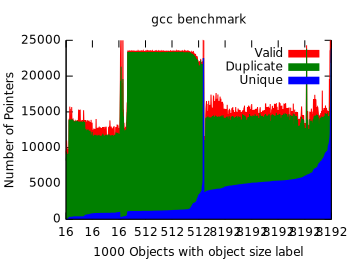
\includegraphics[width=2.8in,height=2.4in,keepaspectratio]{plots/gcc_pointerpattern.pdf}
  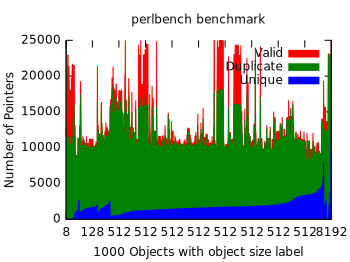
\includegraphics[width=2.8in,height=2.4in,keepaspectratio]{plots/perlbench_pointerpattern.pdf}
  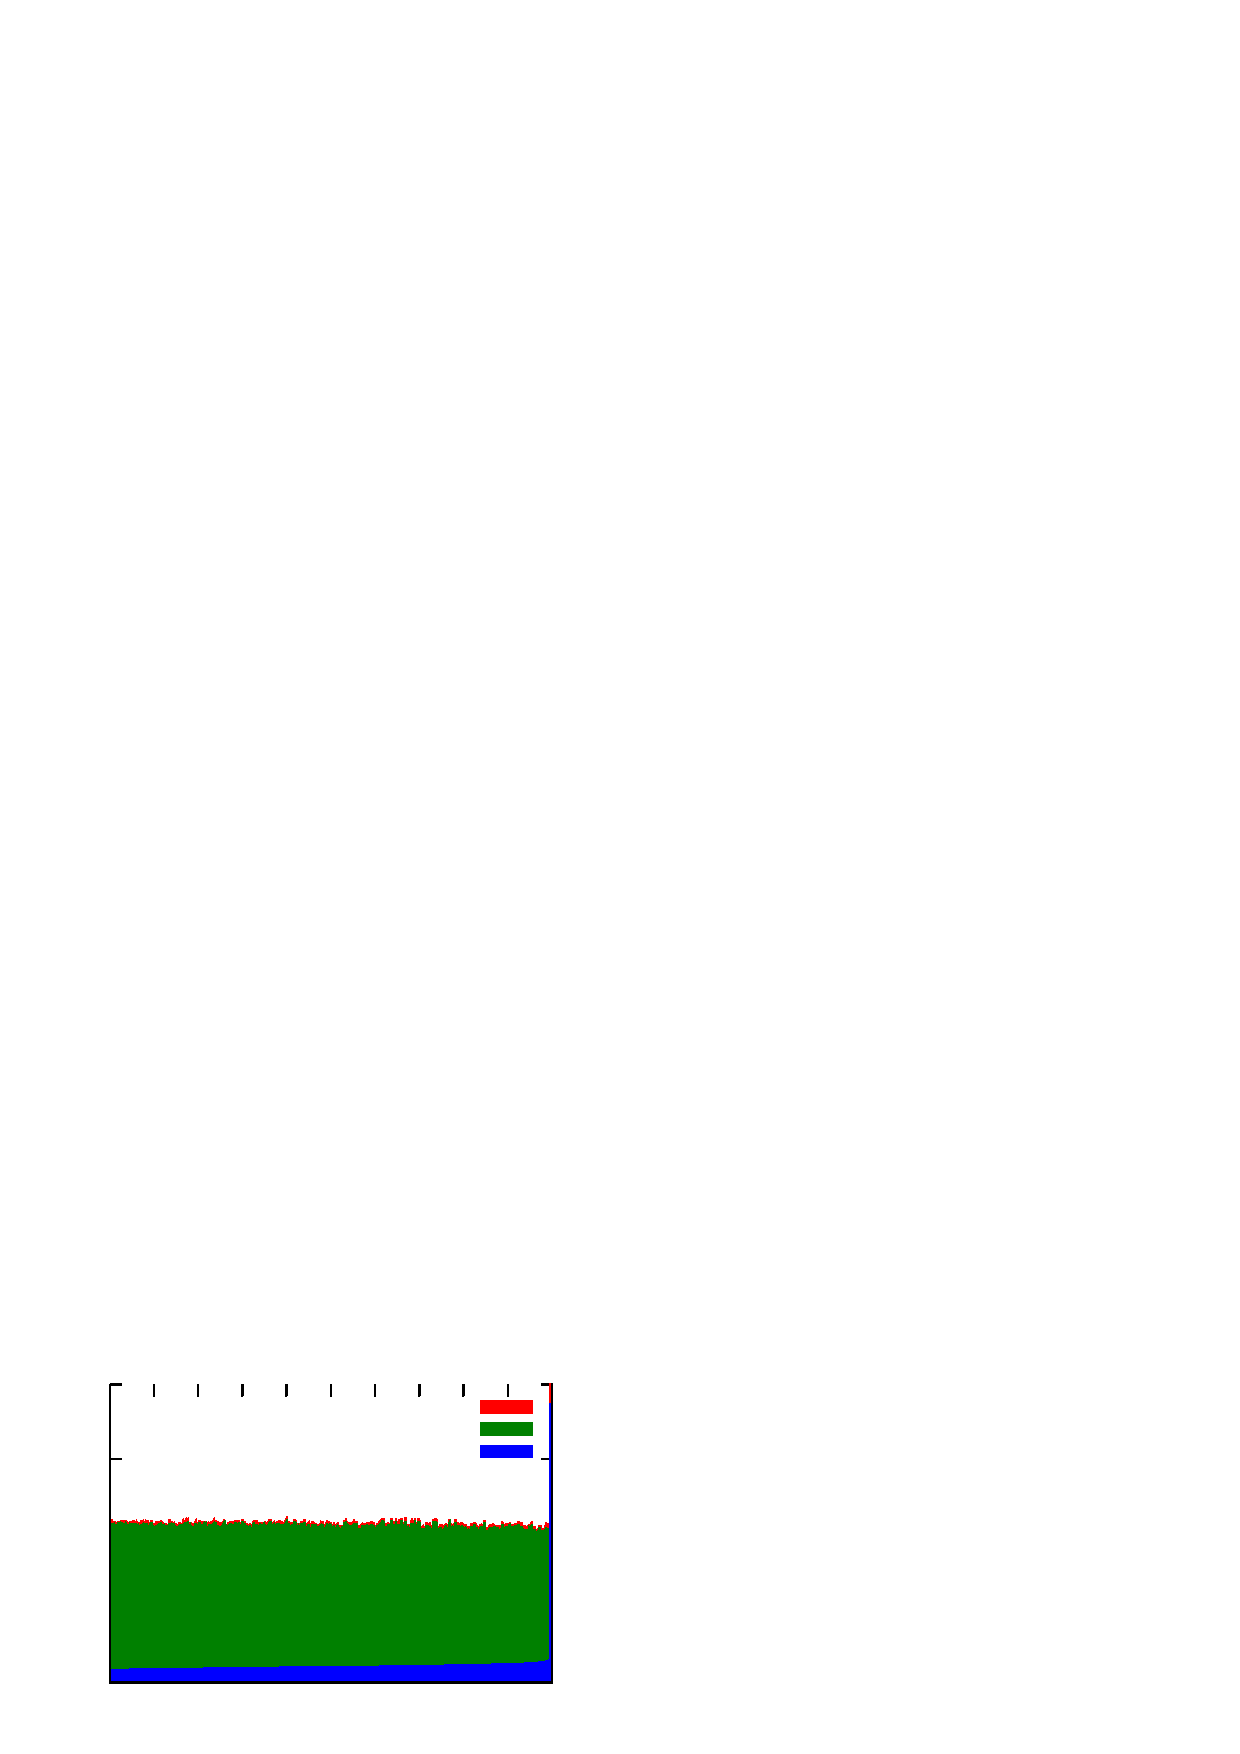
\includegraphics[width=2.8in,height=2.4in,keepaspectratio]{plots/astar_pointerpattern.pdf}
  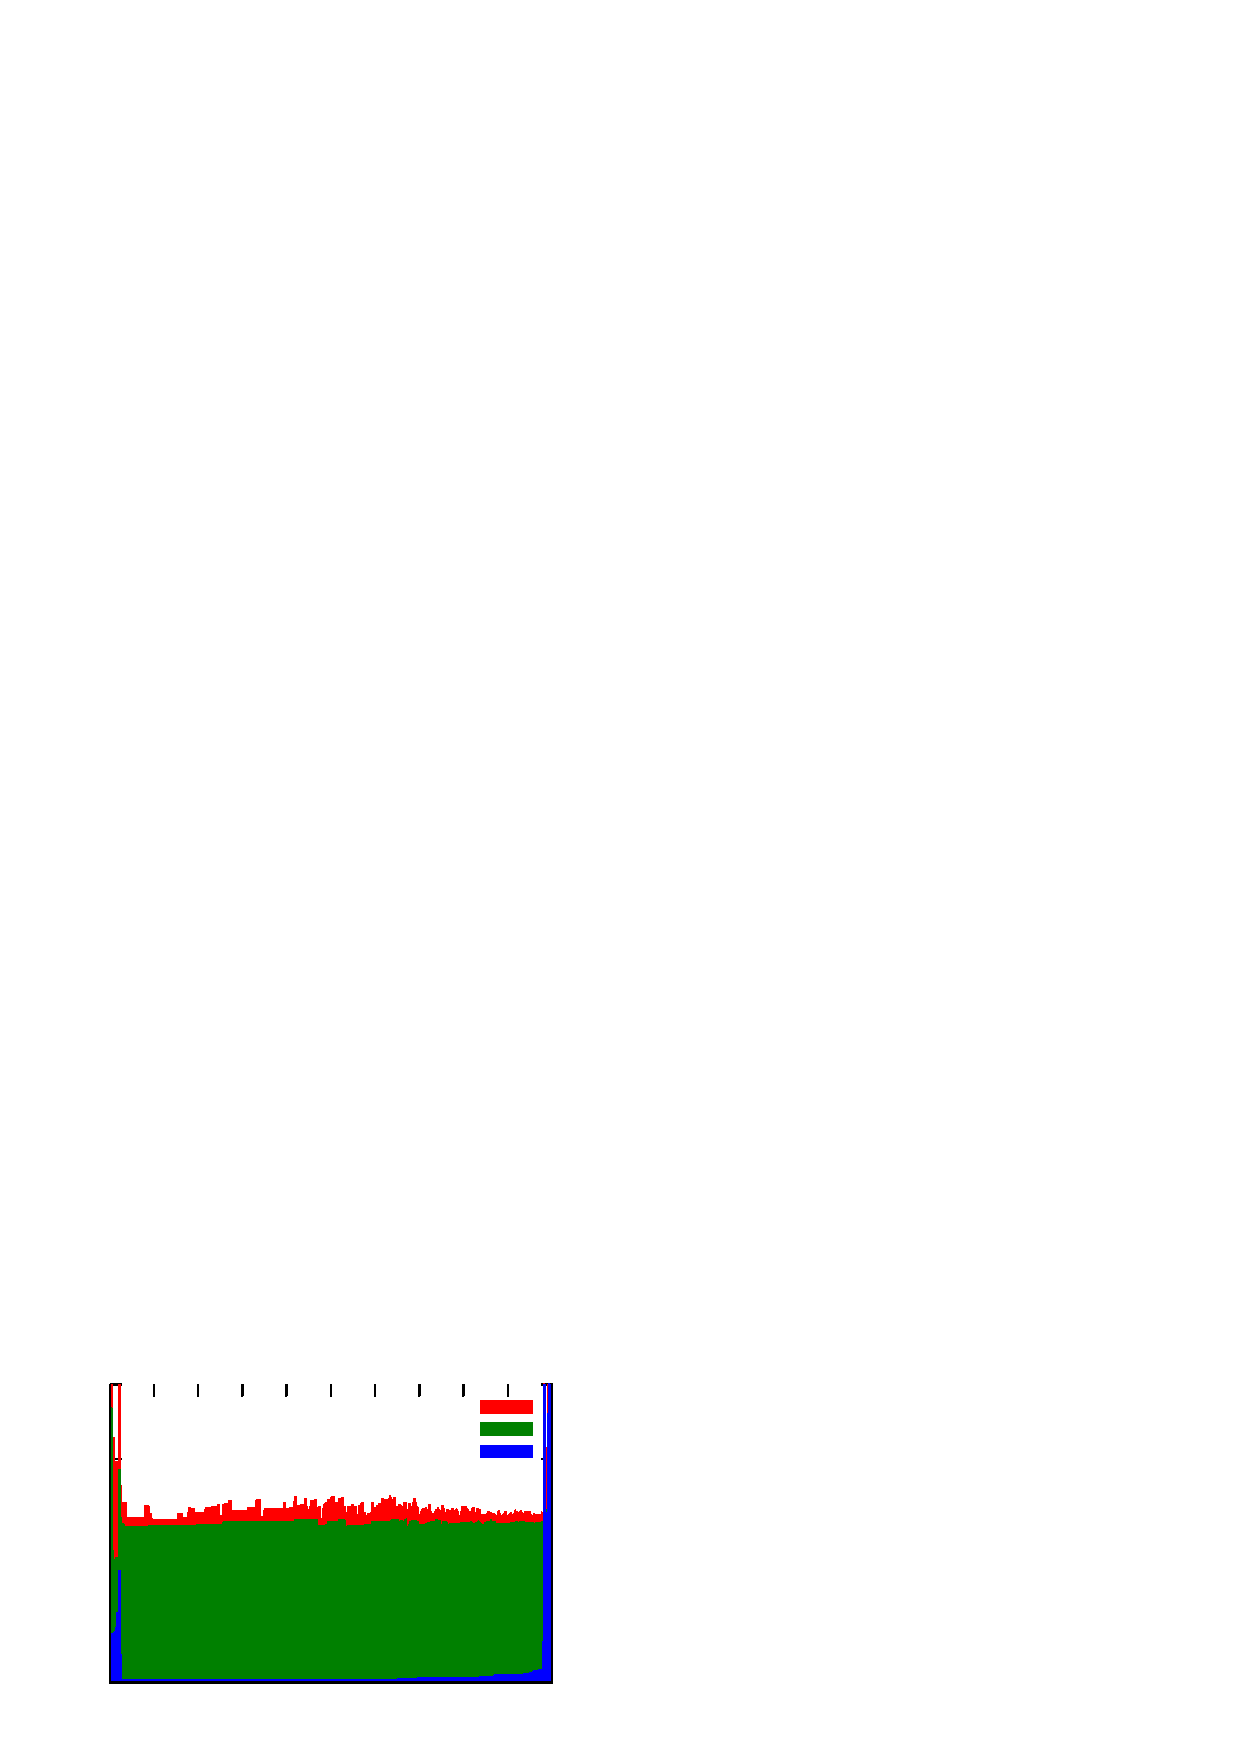
\includegraphics[width=2.8in,height=2.4in,keepaspectratio]{plots/xalancbmk_pointerpattern.pdf}
  
  \caption{Pointer registration pattern for the benchmarks that incur huge overhead. First $1000$ baselog overflow numbers are collected. N-Lookbehind value is $4$. Size of the baselog is kept very high to clearly visualize pattern difference.}
  \label{fig:pointerpattern}
  \vspace{-1em}
\end{figure*} 

Figure~\ref{fig:pointerpattern} shows pointer pattern distribution when a baselog overflow. We collected pointer pattern for first $1000$ objects that have overflown. The graph is plotted with increasing object size. Moreover, we collected statistics for benchmarks that incur huge overhead. Therefore, we chose two C benchmarks (\texttt{gcc} and \texttt{perlbench}) and two C++ benchmarks (\texttt{astar} and \texttt{xalancbmk}). We set baselog size to a very high value, $8K$ (number of pointers). Setting baselog size to a high value makes pattern clearly visible. We used \emph{N}-lookbehind value as $4$. In Figure~\ref{fig:pointerpattern}, red, green and blue area represents \textit{Valid}, \textit{Duplicate} and \textit{Unique} pointers, respectively. All four benchmarks have large number of \textit{Duplicate} pointers for any object size. Even after setting \emph{N}-Lookbehind value to $4$, \textit{Duplicate} pointers count is very high. Increasing value of \emph{N} may decrease \textit{Duplicate} pointers count but it has to trade-off with performance degradation. Furthermore, \emph{Unique} pointers count increases with object size for all the four benchmarks. Therefore, default baselog size should be proportional to the object size. However, it may introduce huge memory overhead. Next, the sum of \textit{Duplicate} and \textit{Unique} pointers represent the total number of pointers in the log. We store at max three pointers per log slot. Therefore, the total number of pointers per log can be at max $8K\ (log size) \times 3 = 24K$. For all the four benchmarks, on an average the total pointers count is above $11000$. In \texttt{gcc}, total pointers count reaches $23K$ for the object size $512$. That is, three times improvement in the memory utilization. Also, \textit{Valid} pointers count is very low for all the four benchmarks. Note, \textit{Valid} pointers count is inflated because pointers that are \textit{Duplicate} and \textit{Valid} are counted more than once. \textit{Valid} pointers count is very low even after counting \textit{Duplicate} and \textit{Valid} pointers more than once. Therefore, we need garbage collection of \textit{Stale} pointers to free the log space. \\

Furthermore, some pointers point to the same object but at different offset. These duplicate pointers may escape \emph{N}-Lookbehind strategy. We introduced one more strategy to remove these duplicate pointers. We compare old pointer value to the new object address range. When pointer points to the same object, we skip pointer registration. This \textit{Duplicate} pointers removal technique not only helps to remove \textit{Duplicate} pointers within a thread but also across threads. This technique removed $20\%\ to\ 25\%$ \emph{Duplicate} pointers for SPEC2006 benchmarks. For this technique, we need old pointer value in run-time tracking function. We slightly changed our static instrumentation pass. We insert run-time tracking function before store instruction instead of after store instruction. In run-time tracking function, we read old pointer value and check whether it still points to the same object. For fast check, we store object bound information in the object metadata. We store lowermost $32$-bits of object root address and object size together in the $64$-bit object metadata field. Therefore, \metalloc{} stores and retrieves $16$ bytes metadata, $8$ bytes for a pointer to a per-Thread log list and $8$ bytes for object information. \\

\subsection{Correctness}
We evaluated \projectname{} correctness on publicly available exploits. We chose following Use-after-Free (Double free) vulnerabilities. \\

\textbf{CVE-2010-­2939}~\cite{OpenSSLCVE}: This is a double free vulnerability in OpenSSL client version OpenSSL1.0.0a and function \texttt{ssl3\_get\_key\_exchange}. It is a highly critical vulnerability that results into denial of service or possible arbitrary code execution. We used exploit with the baseline configuration. It resulted into memory corruption error messages. Furthermore, we compiled OpenSSL1.0.0a with \projectname{}. We tried to exploit the compiled OpenSSL client. However, our system prevented double free. It aborted OpenSSL client due to invalid memory access.
\begin{verbatim}
src/tcmalloc.cc:290] Attempt to free invalid 
pointer 0x80000000022ba510 
./runclient: line 9: 20200 Aborted 
\end{verbatim} 
Above message indicates that our system had invalidated pointer by setting uppermost bit to $1$ when the object was freed first time.
 
\subsection{Memory Overhead}  
% Run-time stats to explain more numbers
\begin{table}[t]
\center
\begin{tabular}{l|*{3}{r}}
	\toprule
	\tablecell{Benchmarks} & \tablecell{Baseline \\RSS} & \tablecell{DangSan \\RSS} & \tablecell{Memory \\Overhead(MB)} \\
	\toprule
	\csvreader[head to column names]{Tables/spec_memory.csv}{}
	{\\\benchmarks & \baselinerss & \dangrss & \extramemory} \\% specify coloumns here
	\bottomrule
\end{tabular}
\caption{Memory overhead for the SPEC2006 benchmarks (MB)}
\label{table:spec_memory}
\end{table}

Table~\ref{table:spec_memory}\ shows memory overhead on SPEC2006 benchmarks introduced by \projectname{}. \texttt{perlbench}, \texttt{omnetpp}, \texttt{xalancbmk} and \texttt{astar} benchmarks have huge memory overhead in gigabytes. Memory overhead also comes from the metadata management scheme, \metalloc{}. \metalloc{} stores and retrieves $16$ bytes metadata for each object. It maintains metadata for all objects (including Stack and Global). We do not track Stack and Global objects. Thus, maintaining $16$ bytes metadata for Stack and Global object can inflate memory overhead numbers. Some defences may not require stack or global metadata management. One of the improvement required in \metalloc{} is to have selective metadata management. We believe that ~\metalloc{} will be used for other defences along with \projectname{}. Another reason for the memory overhead is, we increase one byte for every object allocation to solve \textbf{off-by-one} byte application compatibility issue. However, \texttt{tcmalloc} allocates object with powers of $2$ size. This tremendously increases memory overhead. One improvement to reduce memory overhead is to select additive increase log resize strategy. Table~\ref{table:spec_memory} also represents that increase in memory requirement increases performance overhead. This is directly proportional to the number of pointer propagations and object allocations. 
%\subsection{Performance Analysis}
%\subsection{Correctness}

\section{Limitations and Future Work}
\projectname{} tracks only heap objects. Stack objects can be supported similar to heap objects. \metalloc{} provides uniform way to store and retrieve metadata for stack objects. Static instrumentation has to be changed to insert run-time checks at the start and end of function calls. Moreover, we need to handle \texttt{longjmp} that performs non-local jumps. However, frequent stack object allocations and deallocations incur huge overhead. Furthermore, we conservatively instrument pointer store instructions. We can perform advanced inter-procedural and backward data flow analysis to eliminate stack and global objects accurately. One of the optimization is to avoid instrumentation for simple pointer arithmetic like \emph{p++}. Similar to \freesentry{}, we can move instrumented tracking function outside the loop if the same pointer is used in the loop. Also, we can provide function attribute to opt-out function from being instrumented. 

 

\section{Related Work} \label{relatedwork}
Much work has been done to prevent and detect use of dangling pointers. Mitigation scheme include techniques like static analysis and dynamic analysis. Other schemes propose customized memory allocators, memory error detection tools, safe languages etc. \\

% 1) What is this?
% 2) What are the solutions?
% 3) Explain drawbacks of each?

\textbf{Static Analysis}:
Static analysis performs source code or binary analysis to find memory errors statically.~\cite{feist2014statically}, SLAyer~\cite{berdine2011slayer},  needs inter-procedural pointer or data flow analysis. Static analysis does not cover all possible dangling pointer dereferences because object allocations, deallocations, pointer propagations and dangling pointer dereference can be in different modules, functions and threads. These techniques are not scalable for large applications. In many viable solutions, static analysis is combined with dynamic run-time check to detect Use-after-Free exploits efficiently .\\

\textbf{Dynamic Analysis}.
Dynamic analysis tracks run-time pointer-object relationship. Recent schemes like \dangnull{}~\cite{lee2015dangnull}, \freesentry{}~\cite{younan2015freesentry}, UnDangle~\cite{caballero2012undangle}, CETS~\cite{nagarakatte2010cets}, Address Sanitizer~\cite{serebryany2012addresssanitizer} use run-time information to prevent Use-after-Free exploits. \dangnull{} uses variant of red-black binary tree to efficiently store and retrieve memory object metadata. \dangnull{} has huge average run-time overhead of $80\%$. Moreover, it does not track all pointers (Stack, Global and Heap). \freesentry{} has low average run-time overhead of $25\%$. However, it has no support for multi-threaded applications. That is, it is unclear how much performance overhead \freesentry{} incurs in production servers. UnDangle uses execution trace, taint tracking technique to identify memory locations associated for the same taint. It is useful in software testing. It needs full test coverage to identify all dangling pointers. It does not prevent dangling pointers use during program execution. Address Sanitizer detects memory errors during run-time. It extends compiler infrastructure LLVM to provide memory protection option. It covers most of the memory corruption bugs. However, it has on an average run-time overhead of $73\%$.~\cite{dhurjati2006efficiently} proposed improvements over Electric Fence~\cite{dhurjati2006efficiently}. It uses page protection mechanism to detect dangling pointer deference. It allocates new virtual page for every memory object. It has solved the virtual address space exhaustion problem by mapping multiple virtual pages to same physical page. However, this technique is inefficient for the applications that have large number of object allocations and deallocations.\\

\textbf{Memory Allocators}.
Memory allocators designed to mitigate Use-after-Free vulnerabilities provide transparent solution. Cling~\cite{akritidis2010cling} memory allocator is based on type-safe address reuse technique. Moreover, it does not use free memory for the metadata. Cling prevents type unsafe address reuse but it does not prevent unsafe dangling dereference for the same type object. DieHarder~\cite{novark2010dieharder} memory allocator is a probabilistic approach to find memory errors. It randomize the location of heap objects that makes exploit hard to execute. DieHarder has low overhead but it is probabilistic (i.e. may not cover all dangling pointer dereferences). \\

\textbf{Memory error detectors}.
Valgrind~\cite{nethercote2007valgrind} and Purify~\cite{hastings1991purify} are widely used memory error debugging tools.  Both the tools are used in software testing and debugging. Therefore, its effectiveness depends on the total test coverage. Moreover, Valgrind and Purify incurs huge performance overhead in the order of $10x$. GCCs Mudflap~\cite{eigler2003mudflap} performs dynamic memory access check by maintaining identifier for every allocated object. Checking every memory access incurs huge performance overhead. \\

\textbf{Safe Languages}:
Cyclone~\cite{jim2002cyclone} is a safe dialect of C programming language. It prevents widely present spatial and temporal vulnerabilities of C language. It performs flow analysis and run-time checks. C applications require significant changes to port the application to Cyclone (as it has somewhat different syntax and semantics to simplify static analysis). It uses conservative garbage collection strategy which makes it slower than regular C language. CCured~\cite{necula2005ccured} adds memory safety to the C language by introducing run-time checks. It needs metadata for run-time checks. Porting of C application becomes difficult due to metadata requirement. Similar to Cyclone, CCured uses garbage collection that introduces significant run-time and memory overhead.  

% 1) Prevention techniques using only static analysis
% 2) Prevention techniques using run-time or dynamic analysis
% 3) Customized memory allocators.
% 4) Widely used memory error detector tools, like valgrind.
% 5) Memory safe languages




\section{Conclusion} \label{conclusion}
In this paper, we presented \projectname{}, a fast and efficient lock-less system to detect Use-after-Free exploits in multi-threaded applications. Thread-safety in multi-threaded program incurs prohibitively high run-time overhead. Our design (inspired from Log-structured file system) maintains per-Thread per-Object metadata that eliminates contention between threads. \projectname{} has moderate run-time overhead on CPU intensive benchmarks when all pointers (Heap, Stack and Global) are tracked. It has low throughput degradation for widely used WebServers. Our complete and efficient \projectname{} system can be used for large production applications.

%\projectname{} efficiently detects Use-after-Free exploit in Mul      


\section*{Acknowledgement}
The author would like to thank his mentor and supervisor Erik van der Kouwe, Cristiano Giuffrida for their guidance and valuable assistance.


\bibliographystyle{abbrvnat}
\bibliography{refs}

\end{document}
